\newpage
\section{Grundlagen} \label{Grundlagen}
Fehlender-Text

\subsection{Service Roboter}
In den letzten Jahren haben Service Roboter in verschiedenen Branchen an Bedeutung gewonnen. Ein Grund hierfür ist der technische Fortschritt der Robotik in kombination mit KI, Big Data, Kameras, Sensoren und Spracherkennung \cite[S.~424]{Paluch2020}. Dieser Abschnitt gibt einen kurzen Überblick über Service Roboter im allgemeinen und eine Einführung in die Funktionen der Roboter, die in dieser Arbeit eingesetzt werden. Auch wird das System beschrieben über das der Prototyp mit den Robotern kommunizieren wird.

\subsubsection{Definition}
In wissenschaftlichen Arbeiten werden viele verschiedene Definitionen für Service Roboter genutzt. In dieser Arbeit wird mit der Definition aus der ISO Norm 8373:2021 \cite[Kap.~3]{ISO2021} gearbeitet. Nach dieser handelt es sich bei Service Roboter um Roboter die im privaten oder professionellen Gebrauch nützliche Aufgaben für Menschen oder Equipment erledigen. Hierbei werden Service Roboter außerdem von Industrierobotern und Medizinrobotern abgegrenzt. Die \ac{IFR} \cite{IFR2024} ergänzt die Voraussetzung, dass Service Roboter voll- oder zumindest teilautonom handeln können. Unter dem professionellen Einsatz von Service Robotern versteht man solche, die kommerziell eingesetzt werden \cite[S.~4]{GonzalezAguirre2021}, beispielsweise in den Bereichen Gesundheitswesen, Landwirtschaft oder Tourismus \cite[S.~9]{GonzalezAguirre2021}.

\subsubsection{Einsatzmöglichkeiten}
Service Roboter werden bereits in vielen Bereichen eingesetzt. So gibt es verschiedene Beispiele in denen Service Roboter in Hotels für den Gästeempfang, Check-in und Gepäcklieferung eingesetzt werden. Auch werden Sie an Flughäfen für die Beratung von Reisenden, Scannen von Boardingpässen, Check-in, Bodenreinigung und Patrouilliengänge genutzt. In der Pflege helfen Service Roboter den Pflegern beim Heben von Patienten und durchführen von Übungen mit Patientengruppen. Auch können Roboter in der Pflege angenehme Gespräche starten \cite[S.~425-427]{Paluch2020}. Aufgaben mit geringer kognitiver und emotionaler Komplexität können Service Roboter hierbei vollautonom und ohne Aufsicht durch einen Menschen durchführen \cite[S.~429]{Paluch2020}. Hierbei handelt es sich beispielsweise um Aufgaben wie Staubsaugen, Rasenmähen oder Gepäcklieferung. Für komplexere Aufgaben braucht es die Aufsicht oder Unterstützung von Menschen, wodurch diese nur teilautonom ausgeführt werden.

Service Roboter die im Kontakt mit Kunden eingesetzt werden bieten verschiedene mögliche Vorteile, die aber immer abgewägt werden müssen. Beispielsweise können Roboter Emotionen vorspielen, die von Kunden aber als unauthentisch erkannt werden. Dafür können Roboter durchgängig freundlich sein und können nicht so wie Menschen unter emotionalem Burnout leiden \cite[S.~427]{Paluch2020}. 

\subsubsection{Pudu Roboter}

Wie bereits erwähnt beschäftigt sich diese Arbeit mit Robotern von Pudu. Pudu stellt Service Roboter her, die in der Gastronomie für verschiedene Zwecke eingesetzt werden können. Die Roboter sind auf bestimmte Funktionen spezialisiert. Diese Funktionen sind das Begrüßen und Geleiten von Gästen, das Liefern bestellter Speisen und Getränke, das Zurückbringen dreckigen Geschirs und das Putzen des Bodens \cite{PUDU2024}.

Damit die Roboter diese Funktionen ausführen können müssen sie eigenständig durch komplexe, sich ändernde Umgebungen navigieren. Diese Aufgabe lässt sich in die Positionierung, Wahrnehmung und Routenplanung aufteilen, wobei die Positionierung eine Schlüsselrolle spielt \cite{Nature2022}. Zur Positionierung wird eine eigen entwickelte Version von \ac{VSLAM} eingesetzt. Bevor die Roboter eingesetzt werden, müssen sie mithilfe von \ac{VSLAM} eine Karte ihrer Umgebung erstellen. Auf einer Fläche von 1000 Quadratmetern kann das eine Stunde dauern. Daraufhin kann sich der Roboter mithilfe einer nach oben gerichteten Kamera anhand der Zimmerdecke orientieren. Zur Orientierung brauchen Roboter normalerweise platzierte Markierungen. Diese werden mit der eingesetzten Implementierung von \ac{VSLAM} nicht gerbaucht.\cite{Pudu2023} Mit weiteren Kameras und Sensoren können die Roboter ihre Umgebung wahrnehmen. Mithilfe von KI können die Roboter hierbei Kinder und Senioren erkennen, um sich von ihnen fernzuhalten oder in ihrer Nähe langsamer zu fahren \cite{Nature2022}.

\subsubsection{Bot Control Backend}
Im Rahmen dieser Arbeit wird eine bereits existierende Schnittstelle zwischen den Pudu Robotern und der prototypischen Webanwendung genutzt. Diese Schnittstelle ist das sogenannte \ac{BCB}. In diesem Abschnitt wird die Verbindung zwischen dem \ac{BCB} und den Pudu Robotern erläutert. Im weiteren Verlauf dieser Arbeit wird nicht weiter auf diese Verbindung eingegangen, sondern stattdessen nur auf einzelnen Endpunkte des \ac{BCB}.

Die folgende Abbildung veranschaulicht die Kommunikation zwischen dem Bot Control Backend und den Robotern. So wie die Abbildung, stammen die folgenden Informationen zum Service Framework von Pudu, das zur Kommunikation zwischen Robotern und \ac{BCB} genutzt wird, aus dem SDK Guidance Document von Pudu \cite{PuduSDK}. Das Dokument steht nicht im Internet zur Verfügung und bietet keine genaueren Information zur MQTT basierten Kommunikation zwischen Microservice, PUDU Cloud und Robotern.

\begin{figure}[H]
\caption{Kommunikation zwischen Bot Control Backend und Robotern}
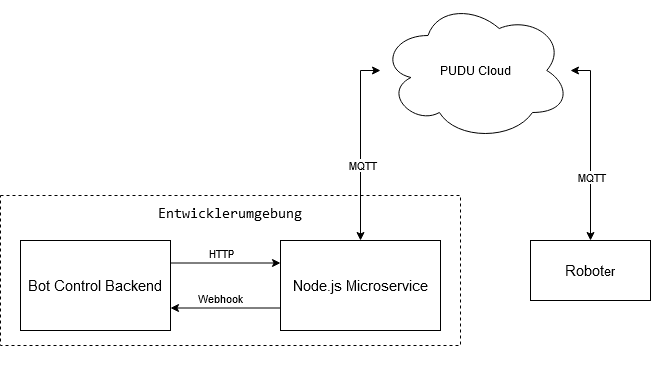
\includegraphics[width=0.9\textwidth]{BotControlBackend Diagramm}
\\
Quelle: In Anlehnung an Pudu \cite[S.~4]{PuduSDK}
\end{figure}

Wie man in der Abbildung sieht hat das \ac{BCB} nur eine direkte Verbindung zum Node.js Microservice, welches wiederum über die PUDU Cloud mit den Robotern kommuniziert. Über \gls{HTTP}-Anfragen an den Node.js Microservice können Befehle verschickt und Daten abgefragt werden. Der Node.js Microservice leitet diese Anfragen via \gls{MQTT} an die PUDU Cloud weiter. Anfragen die nicht an die Roboter weitergeleitet werden müssen, weil die angefragten Daten in der PUDU Cloud liegen, werden auf dem gleichen Weg direkt beantwortet. Muss mit den Robotern kommuniziert werden, dann wird die Anfrage von der PUDU Cloud über \gls{MQTT} an die relevanten Roboter weitergeleitet, die diese dann beantworten. Die Roboter können auch unaufgefordert Ereignisse an das \ac{BCB} kommunizieren. Hierfür muss das \ac{BCB} eine Adresse für einen bestimmten Ereignistyp im Microservice als \gls{Webhook} registrieren. Tritt das entsprechende Ereignis auf, schickt der Roboter diese Information via \gls{MQTT} über die PUDU Cloud an den Microservice. Dieser schickt daraufhin eine HTTP-Anfrage an die registrierte Adresse.

Das \ac{BCB} dient nicht nur als Schnittstelle zu den Pudu Robotern, sondern abstraiert neue Funktionen aus denen die Pudu bietet. Zum einen bietet das \ac{BCB} die Möglichkeit einen Lieferroboter über einen Fahrstuhl zu einem Lieferpunkt in einem anderen Stockwerk zu schicken. Zum anderen kann der Roboter vor einer geschlossenen Tür halten, diese öffnen und dann weiter fahren. Diese beiden Funktionen bietet Pudu nicht.

\newpage
\subsection{Webanwendungen}
Fehlender-Text


\newpage
\subsection{3D Modelle}
Fehlender-Text

\subsubsection{Arten von 3D Modellen}
Fehlender-Text
% Punktwolke und Polygonnetz erklären
% Erwähnen, dass bestimmte Scann/Photogrammetrie (?) Methoden Punktwolken ausgeben
% Diese eignen sich allerdings nicht für die Einbindung zusätzlicher Daten
% Daher Polygonnetze am besten geeignet
% Methoden die Punktwolken erzeugen automatisch ungeeignet

\subsubsection{Generierung}
Fehlender-Text

\paragraph{Fotogrammetrie}
Fehlender-Text

\paragraph{LiDAR Scanning}
Fehlender-Text

\paragraph{Scan2Scene}
Fehlender-Text

\paragraph{Modellierungs-Software}
Fehlender-Text


\subsubsection{Einbindung im Web}
Fehlender-Text

\paragraph{WebGL}
Fehlender-Text

\paragraph{Three.js}
Fehlender-Text

\paragraph{deck.gl}
Fehlender-Text